
\documentclass[a4paper,12pt]{article}
%%%%%%%%%%%%%%%%%%%%%%%%%%%%%%%%%%%%%%%%%%%%%%%%%%%%%%%%%%%%%%%%%%%%%%%%%%%%%%%%%%%%%%%%%%%%%%%%%%%%%%%%%%%%%%%%%%%%%%%%%%%%%%%%%%%%%%%%%%%%%%%%%%%%%%%%%%%%%%%%%%%%%%%%%%%%%%%%%%%%%%%%%%%%%%%%%%%%%%%%%%%%%%%%%%%%%%%%%%%%%%%%%%%%%%%%%%%%%%%%%%%%%%%%%%%%
\usepackage{eurosym}
\usepackage{vmargin}
\usepackage{amsmath}
\usepackage{graphics}
\usepackage{epsfig}
\usepackage{subfigure}
\usepackage{fancyhdr}
%\usepackage{listings}
\usepackage{framed}
\usepackage{graphicx}

\setcounter{MaxMatrixCols}{10}
%TCIDATA{OutputFilter=LATEX.DLL}
%TCIDATA{Version=5.00.0.2570}
%TCIDATA{<META NAME="SaveForMode" CONTENT="1">}
%TCIDATA{LastRevised=Wednesday, February 23, 2011 13:24:34}
%TCIDATA{<META NAME="GraphicsSave" CONTENT="32">}
%TCIDATA{Language=American English}

\pagestyle{fancy}
\setmarginsrb{20mm}{0mm}{20mm}{25mm}{12mm}{11mm}{0mm}{11mm}
\lhead{MA4128} \rhead{Mr. Kevin O'Brien}
\chead{Advanced Data Modelling}
%\input{tcilatex}


% http://www.norusis.com/pdf/SPC_v13.pdf
\begin{document}

%----------------------------------------------------------%
% http://www2.statistics.com/resources/glossary/h/hclusteran.php

% http://mlsc.lboro.ac.uk/resources/statistics/Clusteranalysis.pdf

\section{Cluster Methods}
\begin{itemize}
\item Having selected how we will measure distance, we must now choose the clustering algorithm, i.e. the rules that govern between which points distances are measured to determine cluster membership. 
\item There are many methods available, the criteria used differ and hence
different classifications may be obtained for the same data. This is important since it tells us that, although cluster analysis may provide an objective method for the clustering of cases, there can be subjectivity in the choice of method. 

\item The linkage distances are calculated by SPSS. The goal of the clustering algorithm is to join objects together into successively larger clusters, using some measure of similarity or distance. SPSS provides seven clustering algorithms, the most commonly used one being  \textbf{\textit{Ward's method}}.

\item SPSS provides several alternative methods for determining a summary measure of distance when a cluster has multiple cases in the cluster.
\item   The SPSS options for the clustering method are Between-groups linkage, Within-groups linkage, Nearest neighbor, Furthest neighbor, Centroid clustering, Median clustering, and Ward's method.

\end{itemize}



\subsection{Nearest Neighbour Method} 
%(\textit{Also known as the single linkage method}).\\


\begin{itemize}
	\item In this method the distance between two clusters is defined to be the distance between
	the two closest members, or neighbours. 
	\item For the \textbf{nearest neighbor} or \textbf{single linkage} method, the dissimilarity between cluster A and cluster B is represented by the minimum of all possible distances between the cases in cluster A and the cases in cluster B.
		
	\item The distance between two clusters corresponds
	to the shortest distance between any two members in the two clusters.
	\begin{figure}[h!]
		\begin{center}
			% Requires \usepackage{graphicx}
			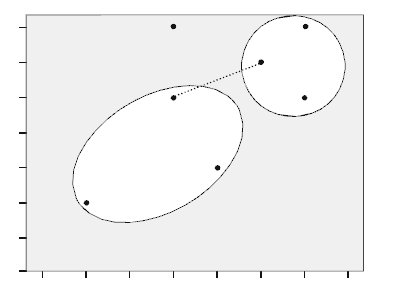
\includegraphics[scale=0.4]{images/Link1.jpg}\\
			\caption{Single linkage (nearest neighbor)}
		\end{center}
	\end{figure}	
	\item This method is relatively simple but is often
	criticised because it doesn’t take account of cluster structure and can result in a problem
	called \textbf{chaining} whereby clusters end up being long and straggly. 
	\item However, it is better
	than the other methods when the natural clusters are not spherical or elliptical in shape.
\end{itemize}


\subsection{Furthest Neighbour Method} 
\begin{itemize}	
	\item For the \textbf{furthest neighbor} or \textbf{complete linkage} method, the dissimilarity between cluster A and cluster B is represented by the maximum of all possible distances between the cases in cluster A and the cases in cluster B.
	\item 
	In this case the distance between two clusters is defined to be the maximum distance
	between members, i.e. the distance between the two subjects that are furthest apart.
\item This method tends to produce compact clusters of similar size but, as for the nearest
	neighbour method, does not take account of cluster structure. It is also quite sensitive
	to outliers.

	\begin{figure}[h!]
		\begin{center}
			% Requires \usepackage{graphicx}
			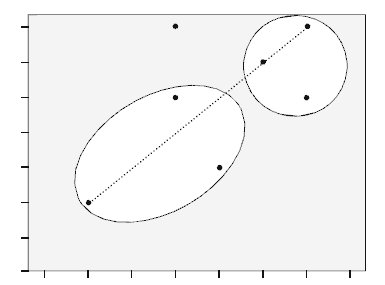
\includegraphics[scale=0.4]{images/Link2.jpg}\\
			\caption{Complete linkage (furthest neighbor)}
		\end{center}
	\end{figure}
		\item  This is the oppositional approach to single
		linkage assumes that the distance between two clusters is based on the longest
		distance between any two members in the two clusters.
\end{itemize}



\subsection{Average (between groups) Linkage Method }
(\textit{sometimes referred to as UPGMA}).\\
\begin{itemize}
\item For the \textbf{between-groups linkage} or average linkage method, the dissimilarity between cluster A and cluster B is represented by the \textbf{\textit{average of all the possible distances}} between the cases in cluster A and the cases in cluster B. 
% \item The distance between two clusters is calculated as the average distance between all pairs
% of subjects in the two clusters. 
\item This is considered to be a fairly robust method.
% \item : The distance between two clusters is defined as the average distance between all pairs of the two clusters’ members.
\begin{figure}[h!]
	\begin{center}
		% Requires \usepackage{graphicx}
		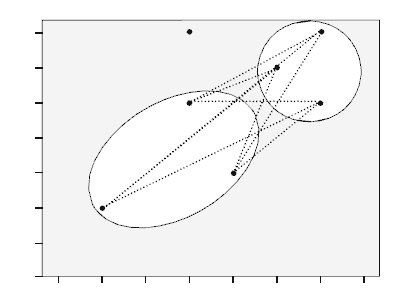
\includegraphics[scale=0.4]{images/Link3.jpg}\\
		\caption{Average linkage}
	\end{center}
\end{figure}
\end{itemize}




\subsection{Centroid Method}
\begin{itemize}
	\item For the \textbf{centroid clustering} method, the dissimilarity between cluster A and cluster B is represented by the \textbf{\textit{distance between the centroid}} for the cases in cluster A and the centroid for the cases in cluster B.  
	\item  In this approach, the geometric center (centroid) of each cluster is
	computed first. Then the distance between the two clusters equals the distance between
	the two centroids.
	\item Note that this distance is not mathematically equivalent to the average of the distances used in the average linkage method. \\ \textit{Also note the SPSS warning below about using squared Euclidean distance rather than Euclidean distance for this procedure}.

	\begin{figure}[h!]
		\begin{center}
			% Requires \usepackage{graphicx}
			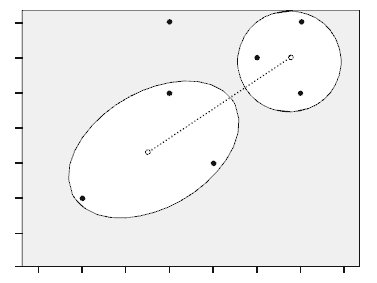
\includegraphics[scale=0.4]{images/Link4.jpg}\\
			\caption{centroid}
		\end{center}
	\end{figure}
%	\item Here the centroid (mean value for 
%	each variable) of each cluster is calculated and the
%	distance between centroids is used. Clusters whose centroids are closest together are
%	merged. 
	\item This method is also fairly robust. 
\end{itemize}

\subsection{Median Clustering}

\begin{itemize}
	\item 
	For the \textbf{median clustering} method, the dissimilarity between cluster A and cluster B is represented by the distance between the SPSS determined median for the cases in cluster A and the median for the cases in cluster B.  See the message in the note above about using squared Euclidean distance rather than Euclidean distance for this method.
	
\end{itemize}
	
%	
%	\begin{framed}
%		The squared Euclidean measure should be used when the CENTROID, MEDIAN, or WARD cluster method is requested.
%	\end{framed}
	


\subsection{Ward’s method: Within-Groups linkage method}
\begin{itemize}
	
	\item For the \textbf{within-groups linkage} method, the dissimilarity between cluster A and cluster B is represented by the average of all the possible distances between the cases within a single new cluster determined by combining cluster A and cluster B.
	 \item \textbf{Important:} For a cluster the sum of squares is the sum of squared deviations of each case from the centroid for the cluster.  The error sum of squares is the total of these for all clusters. 
	\item \textbf{Important:} In this method all possible pairs of clusters are combined and the sum of the squared
	distances within each cluster is calculated. This is then summed over all clusters. The
	combination that gives the lowest sum of squares is chosen. 

	\item The dissimilarity between cluster A and cluster B is represented by the “loss of information” from joining the two clusters with this loss of information being measured by the increase in error sum of squares.  
	\item When selecting clusters to join, the two clusters among all possible combinations that have the minimum increase in error sum of squares are selected.  
	%See the note above about using squared Euclidean distance rather than Euclidean distance for this method.
		\item This method tends to
		produce clusters of approximately equal size, which is not always desirable. It is also
		quite sensitive to outliers. Despite this, it is one of the most popular methods, along
		with the average linkage method.
\end{itemize}	






%\subsection{Ward's Method}
%This method is distinct from other methods because it uses an \textbf{\textit{analysis of variance}} approach to evaluate the distances between clusters. In general, this method is very efficient.
%
%Cluster membership is assessed by calculating the total sum of squared deviations from the mean of a cluster. The criterion for fusion is that it should produce the smallest possible increase
%in the error sum of squares.
%
%
%
%\subsection{Ward's Linkage}
%
%Ward's linkage is a method for hierarchical cluster analysis . The idea has much in common with analysis of variance (ANOVA). The linkage function specifying the distance between two clusters is computed as the increase in the "error sum of squares" (ESS) after fusing two clusters into a single cluster. Ward's Method seeks to choose the successive clustering steps so as to minimize the increase in ESS at each step.



%\subsection{Linkage methods}
%\begin{itemize}
%	\item  Single linkage (minimum distance)
%	\item  Complete linkage (maximum distance)
%	\item  Average linkage
%\end{itemize}

%http://www.rdg.ac.uk/~aes02mm/supermarket.sav

\begin{figure}[h!]
\centering
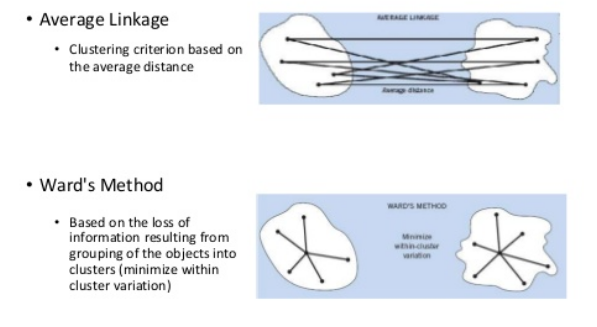
\includegraphics[width=0.7\linewidth]{images/wardlinkage}

\end{figure}


\begin{itemize}

\item A commonly used approach in hierarchical clustering is \textbf{\textit{Ward’s linkage method}}.
This approach does not combine the two most similar objects successively. Instead,
those objects whose merger increases the overall within-cluster variance to the
smallest possible degree, are combined. 
\item If you expect somewhat equally sized
clusters and the data set does not include outliers, you should always use Ward’s
method.

\item We will use the Ward's linkage method for laboratory exercises.
\end{itemize}
\newpage
\subsection{Summary}
\begin{itemize}


\item Each of these linkage algorithms can yield totally different results when used on the same data set, as each has its specific properties. 
\item As the single linkage algorithm is based on minimum distances, it tends to form one large cluster with the other clusters containing only one or few objects each. We can make use of this \textbf{\textit{chaining effect}} to detect outliers, as these will be merged with the remaining objects – usually at very large distances – in the last steps of the analysis. Generally, single linkage is considered the most versatile algorithm.
\item 
Conversely, the complete linkage method is strongly affected by outliers, as it is based on maximum distances. Clusters produced by this method are likely to be rather compact and tightly clustered.
\item  The average linkage and centroid algorithms tend to produce clusters with rather low within-cluster variance and similar sizes. However, both procedures are affected by outliers, though not as much as complete linkage.

\item \textbf{Important:} An understanding of linkage method's other than than Ward method will be expected in the end of year examination.
\end{itemize}



%----------------------------------------------------------%
% http://www2.statistics.com/resources/glossary/h/hclusteran.php

% http://mlsc.lboro.ac.uk/resources/statistics/Clusteranalysis.pdf


%\subsection{Ward's Method}
%This method is distinct from other methods because it uses an \textbf{\textit{analysis of variance}} approach to evaluate the distances between clusters. In general, this method is very efficient.
%
%Cluster membership is assessed by calculating the total sum of squared deviations from the mean of a cluster. The criterion for fusion is that it should produce the smallest possible increase
%in the error sum of squares.
%
%
%
%\subsection{Ward's Linkage}
%
%Ward's linkage is a method for hierarchical cluster analysis . The idea has much in common with analysis of variance (ANOVA). The linkage function specifying the distance between two clusters is computed as the increase in the "error sum of squares" (ESS) after fusing two clusters into a single cluster. Ward's Method seeks to choose the successive clustering steps so as to minimize the increase in ESS at each step.

\end{document}
